%%Berichtvorlage für EDBV WS 2014/2015

\documentclass[paper=A4, deutsch]{scrartcl}
\usepackage[ngerman]{babel}
\usepackage[utf8]{inputenc}
\usepackage{algorithmic}
\usepackage{algorithm}
\usepackage{graphicx}
\usepackage{amsmath,amssymb}
\usepackage{subcaption}
\captionsetup{compatibility=false}
\usepackage{multirow}
\usepackage{color}
\usepackage[]{geometry}
\usepackage{textcomp}
\usepackage{soul}

\newcommand\tab[1][1cm]{\hspace*{#1}}

\begin{document}


%%------------------------------------------------------
%% Ab hier tragt ihr eure Daten und Ergebnisse ein:
%%------------------------------------------------------

\title{Lib-Indexer} %%Projekttitel hier eintragen

\subtitle{EDBV WS 2019/2020: AG\_C\_3} %%statt XX Arbeitsgruppenbezeichnung hier eintragen (zB.: A1)


%%Namen und Matrikelnummern der Gruppenmitglieder hier eintragen
\author{Anand Eichner (11808244)\\
Laurenz Edmund Fiala (11807869)\\
Anna Nieto-Berezhinskaya (01223066)\\
Aleksandar Vucenovic (01635282)}



%%------------------------------------------------------

\maketitle


%%------------------------------------------------------
\section{Gewählte Problemstellung}
\subsection{Ziel}
Das Projekt soll Bücher in einem Bücherregal erkennen, in Bücher-Koordinaten umwandeln und nach ihrem Label abspeichern.

\subsection{Eingabe}
JPG-Bild eines Bücherregals mit Büchern, auf denen eindeutige TU-Bibliotheks-Labels (schwarz-auf-weiß) kleben.

\subsection{Ausgabe}
visuell:\\
\\
\begin{figure}[H]
 \centering
 \includegraphics[width=0.4\textwidth]{input.jpg}
 \caption{Input-Bild}
 \label{fig:img}
\end{figure}


\noindent textuell:\\
Strukturierte Klartext-Datei mit Inhalt:
\begin{itemize}
  \item Standort der Bücher (in Büchern zum Ursprung - links-oben)
  \item Vier Pixel-Vektoren, die ein Label in einem Viereck umschließen
\end{itemize}

\subsection{Voraussetzungen und Bedingungen}
\begin{itemize}
  \item Die Bücher müssen gerade (+/- 5°) stehen.
  \item Das Bild darf nicht mehr als 30° von der Waagrechte abweichen.
  \item Das Bild muss eine für die Texterkennung der Labels ausreichende Auflösung aufweisen (Abhängig von der Entfernung).
  \item Das Bild muss farbig sein.
  \item Das Bild muss ausreichend hell sein. 
  \item Ein Weißabgleich muss durchgeführt worden sein.
\end{itemize}

Neue Anforderungen:
\begin{itemize}
  \item Der Hintergrund der Labels muss weiß sein (Intensität muss über dem globalen Otsu-Threshold liegen)
\end{itemize}

\subsection{Methodik}
Methodik- Pipeline
\begin{enumerate}
	\item Hough-Transformation\\
		\textit{Finden der Regalfächer zum Korrigieren der Perspektive}
	\item Persprektivenkorrektur\\tuwe
		\textit{Mittels Transformationsmatrix aus HT berechnet}
	\item Eckenerkennung\\
		\textit{Finden der Ecken von Labels}
	\item Integral imaging\\
		\textit{Finden von Labels innerhalb eines Akzeptanzbereichs, es werden nur Bereiche zwischen verschiedenen, zuvor erkannten, Ecken überprüft}
	\item Eigene Heuristik\\
		\textit{Einordnen von Labels in Buch-Koordinaten}
	\item Optical Character Recognition\\
		\textit{Erkennen von Text auf den Labels in den zuvor erkannten Bereichen}
\end{enumerate}

\subsection{Evaluierungsfragen}
\textbf{Interaktion zwischen den Komponenten:}
\begin{itemize}
	\item \textit{Werden die Regalfächer korrekt erkannt?}\\
		  Voraussetzungen:\tab Seite der Regalfächer, die zur Kamera zeigt, ist schwarz.\\
		  Ergebnis:\tab[2.2cm] An jedem Fach liegt eine Gerade an.
	\item \textit{Wird die Perspektive korrekt angepasst?}\\
		  Voraussetzungen:\tab Korrekte Geraden der Regalfächer.\\
		  Ergebnis:\tab[2.2cm] Bücher und Labels sind im Bild weitestgehend rechteckig.
	\item \textit{Werden alle Labels erkannt?}\\
		  Voraussetzungen:\tab Perspektivenkorrigiertes Bild\\
		  Ergebnis:\tab[2.2cm] Bounding-Boxes der gefundenen Labels
	\item \textit{Sind die Bounding Boxes der gefundenen Labels korrekt? Ist der gesamte Text darin enthalten?}\\
		  Voraussetzungen:\tab Korrekt erkanntes Label oder ein false-positive.\\
		  Ergebnis:\tab[2.2cm] Vier Vektoren, die den gesamten Text umschließen (und nicht mehr). Bei false-positives ist das Ergebnis nicht relevant, jedoch sollte es nicht zu groß sein (z.B. das gesamte Bild überdecken).
	\item \textit{Werden die Labels korrekt in Bücher-Koordinaten umgewandelt?}\\
		  Voraussetzungen:\tab Bounding Boxes der Labels sind korrekt.\\
		  Ergebnis:\tab[2.2cm] Bücher-Koordinatensystem als 2D-Array mit Ursprung links-oben.
	\item \textit{Werden die Labels der TU-Bibliothek korrekt gelesen und in Text umgewandelt?}\\
		  Voraussetzungen:\tab Label Bounding-Boxes wurden korrekt berechnet (enthalten keinen unnötigen Text).\\
		  Ergebnis:\tab[2.2cm] String-Repräsentation des Labels. Erwartete Korrektheit: $>$ 90\% für typische Datensätze.
	\item \textit{Wird die Wahrscheinlichkeit der Label-Korrektheit angemessen berechnet?}\\
		  Voraussetzungen:\tab Korrekt in Text umgewandeltes Label.\\
		  Ergebnis:\tab[2.2cm] Floating-point Wert im Intervall [0, 1]. Alle Labels mit Wahrscheinlichkeit 0 wurden entfernt.
\end{itemize}

\subsection{Zeitplan}
\begin{table}[H]
	\centering
		\begin{tabular}{|c|c|c|}
		\hline
		Meilenstein & abgeschlossen am & Arbeitsaufwand in h\\
		\hline
		Prototyp & 10.11. & 30\\
		\hline
		Hough-Transformation & \st{17.11.} 20.12. & \st{50} 2\\
		\hline
		Perspektivenkorrektur & \st{17.11.} 23.12. & \st{6} 20\\
		\hline
		Labelerkennung & \st{25.11.} 14.11. & 25\\
		\hline
		Labelerkennung - Verbesserungen & \st{25.11.} 5.1. & 30\\
		\hline
		Labels in Buch-Koordinaten & \st{1.12.} 4.1. & \st{4} 0.2\\
		\hline
		Optical Character Recognition & \st{10.12.} 3.1. & \st{110} 40\\
		\hline
		Labels filtern & \st{15.12.} nicht abgeschl. & \st{6} nicht abgeschl.\\
		\hline
		Daten in Output-Format umwandeln & 5.1. & \st{4} 0\\
		\hline
		Tests & \st{18.12.} 5.1. & 5\\
		\hline
		Evaluierung & {20.12.} 5.1. & \st{5} 4 \\
		\hline
		\end{tabular}
\end{table}
%%------------------------------------------------------

%%------------------------------------------------------
\section{Arbeitsteilung}
\begin{center}
  \begin{tabular}{ |l | l | }
    \hline
  Name & Tätigkeiten\\
    \hline
    	Anna Nieto-Berezhinskaya & Harris Eckendetektor (zu feinfühlig und kann\\
    	&deshalb nicht eingesetzt werden)\\
		\hline
		Anand Eichner & houghTransform (+ lokale Funktionen), PerspectiveCorrection\\
		&(+ lokale Funktionen),\\
		\hline
		Laurenz Edmund Fiala & label\_detection (+ lokale Funktionen)\\
		\hline
		Aleksandar Vucenovic & ocr (+ locals), NCC, SSD\_naive\\
		& (+ lokale Funktionen) preprocessing (+ lokale Funktionen)\\
		\hline
  \end{tabular}
\end{center}

%%------------------------------------------------------

%%------------------------------------------------------
\section{Methodik}

\subsection{Perspektivenkorrektur}
Im Vorverarbeitungsschritt wird das Eingabebild in ein Graustufenbild umgewandelt und mit einem vertikalen und einem horizontalen Sobelfilter convoluted um Kantenbilder zu erhalten, dann wird der Betrag dieser Werte genommen um Kanten in beide Richtungen zu finden. Um dem Rauschen im Bild entgegenzuwirken werden alle verbundobjekte unter einer bestimmten Größe ausgefiltert um nur lange Kanten zu behalten. Bei den Vertikalen werden zusätzlich nur die 20 größten Verbundobjekte ausgewählt um dem Rauschen durch die vielen Vertikalen entgegenzuwirken.\\
Die beiden Kantenbilder werden mit hilfe einer Hough-Transformation in den Parameterraum transformiert. Von dort werden folglich einige Maxmima ausgelesen um einige Geraden im Bild zu ermitteln.\\
Aus den Linienscharen werden jeweils zwei Vertikale und zwei Horizontale Ausgewählt um ein Rechteck im Raum darzustellen. Die vier Eckpunkte dieses Rechtecks werden vor der geometrischen Verzerrung perspektivisch Korrekt hochskaliert um die unnötige erstellung redundanter Daten zu verhindern. Mit den skalierten Eckpunkten und den eigentlichen Eckpunkten des Bildes wird nun eine perpsektivische Transformationsmatrix gebildet und auf das Bild angewendet.\\

\subsection{Optical Character Recognition}
\textbf{Image Thresholding (Adaptive)}\\
Das Binarizing des Labels fungiert als Noise Reduktion, zusätzlich ermöglicht es Template Matching mit weiß/schwarzen Bitmaps, da es ein schwarz/weiß Bild zurückliefert.\\
\\
\textbf{Dilation}\\
Dilation ermöglicht eine korrekte Regionproperties Funktion, da es die Löcher in den Components füllt, und diese damit sauber verbindet.\\
\\
\textbf{Regionprops}\\
Regionprops gibt uns die Centrtoids und Bounding boxes von collected components, die in unserem Fall potentielle character sind. Die Methode wird benutzt um die Charakter zu segmentieren, in dem man das Originalbild mit den Koordinaten der Bounding Boxes cropped. Zustätzlich verschafft es uns eine Sortiermethode, mithilfe der Centroids können wir die Wörter nämlich richtig von links oben nach rechts unten sortieren,
da Centroids die XY-Koordinaten der Mitte eines Buchstabens im Bild liefert.\\
\\
\textbf{Prewitt Edge-Detection}\\
Prewitt Edge-Detection wird als preprocessing step für die Dilation und Hough Transformation genutzt, da diese ein Kantenbild als Eingabe brauchen und Prewitt dieses liefert.\\
\\
\textbf{Normalized Cross Correlation (Template Matching)} \cite{nip}\\
Der nxcorr/NCC Algorithmus ist ein sehr weit verbreiteter Algorithmus für das Template Matching. In Matlab selbst ist er als normxcorr2-Funktion durchführbar. 
Er wird verwendet, um die Korrelation zwischen template und original image zu finden, und normalisiert um richtige Ergebnisse unabhängig von Brightness-Unterschieden zu liefern. Das Ergebnis ist eine Korrelationsmatrix, die Werte zwischen -1 und 1 enthält, wobei 0 die kleinste Korrelation repräsentiert und 1 die größte (-1, falls das Original oder Template negiert ist). Wir suchen das globale Maxima in der Matrix, da es den besten Korrelationswert liefert, und vergleichen diesen mit allen Werten der Templates. Das Template mit dem größten Korrelationswert wird schließlich als matched character weitergegeben.\\
\\
\textbf{Sum of Squared Differences (Template Matching)}\\
Der SSD Algorithmus wird auch, wie der nxcorr2-Algorithmus, zum Template Matching verwendet. Der SSD Algorithmus beruht darauf, dass, wenn man ein Template über das Originalbild legt, und die Summe der quadrierten Differenzen der Pixelwerte bildet, ein möglichst kleiner Wert bei einem Match herauskommen sollte (da sich die Werte sehr ähnlich sein müssen). Wir haben eine naivere Variante implementiert, da unser Template und Bild immer gleich groß sind und immer beide Bilder die Buchstaben zur Gänze umschließen. Daher müssen wir keine Regionen absuchen und Offsets ausprobieren.\\
%%------------------------------------------------------
\\

\subsection{Label Detection}

Um die Labels zu erkennen, haben wir uns aufgrund der verschiedenen Label-Dimensionen am Anfang des Projekts dazu entschieden, mittels Integral Imaging (Summed Area Table) zu bestimmen, ob ein Bereich als Label gelten kann oder nicht.\\
Der Prototyp war auch recht erfolgversprechend. Jedoch sind wir im Verlauf des Projekts auf einige Limitationen bei dieser Herangehensweise gestoßen.\\
Es hat sich herausgestellt, dass es oft nicht ganz trivial ist, bei verschiedenen Auflösungen die korrekten Ecken mit dem Harris-Eckendetector zu finden. Hier spielt das Preprocessing, welches ein einfacher Gaußfilter ist, eine große Rolle. Auch die Größe des Gauß-Konvolutionskernels für den Harris-Detektor ist wichtig. Aufgrund von Zeitmangel gegen Ende des Projekts, konnten diese Werte leider nicht mehr so genau bestimmt werden und deshalb ist das Ergebnis leider nicht so genau, wie eigentlich möglich bzw. gewünscht.\\
\\
\textbf{Harris-Eckendetektor} \cite{harris}\\
Der Harris-Eckendetektor wird genutzt, um die Ecken der einzelnen Labels zu erkennen.
Ursprünglich war geplant, diese Methode selbst zu implementieren, jedoch war die selbst implementierte Variante zu sensibel und das konnte aufgrund von fehlenden Projektmitgliedern nicht mehr ausgebessert werden.\\
\\
\textbf{Summed Area Table / Integral Imaging} \cite{integralimg}\\
Das Integral Imaging wird benutzt, um die Intensität der einzelnen Label-Kandidaten effizient berechnen zu können. Im Programmverlauf wird das genutzt, um das Verhältnis von dunken zu hellen Bildabschnitten zu berechenen und damit bestimmen zu können, ob ein Bereich als Label gelten kann oder nicht.\\
\\
\textbf{Otsu-Threshold} \cite{otsu}\\
Es wird ein globaler Threshold benötigt um Labels vom Hintergrund abzugrenzen. Das Integral Image beruht auf dem Ergebnis der Bildmaske dieses Thresholds. Ein Otsu-Threshold eignet sich sehr gut um dynamisch in jedem Bild einen akzeptablen Threshold zu ermitteln.\\
Der Threshold wird auch lokal pro Label-Kandidat angewandt, um den oft sehr hellgrauen Text vom Hintergrund (dem Label) abzugrenzen. Damit ist das Ergebnis des Programms wesentlich zuverlässiger.


%%------------------------------------------------------

%%------------------------------------------------------
\section{Implementierung}
\subsection{Main}
Um das Framwork auszuführen muss main.m mit dem Pfad zum Bild als einziges Argument ausgeführt werden. Die main Funktion gibt dann den json String zurück.\\
\textit{Beispielaufruf:} \texttt{main('Dataset/01.jpg')}\\
\\
\subsection{Perspektivenkorrektur}
Für die Perspektivenkorrekur ist die PerspectiveCorrection.m Datei zuständig. Diese nutzt einige Builtins für das Preprocessing und eine selbstgeschriebene Implementierung der Hough-Transformation (houghTransform.m). Zum Skalieren der Eckpunkte wurden einige Funktionen implementiert um geometrische Operationen mit Linien in Parameterform durchzuführen. Bei der Hough-Transform wird nur ein Wertebereich von -30 bis +30 Grad genutzt um den Parameterraum möglichst klein zu halten. Weiters wird nur nach 5 Maxima gesucht, dies bietet ein gutes Mittelding zwischen schlechten Ergebnissen und zu wenigen Ergebnissen. Es werden bei den Vertikalen Kanten die jeweils 20 Größten behalten dies bietet auch hier wieder ein gutes Mittelding zu viel Rauschen und einer zu geringen Chance eine gute Kante zu erhalten.\\
\\
\subsection{Label Detection}
Die Erkennung der Labels wird in label\_detection.m gehandhabt.\\
Zuerst werden mit einem Harris-Eckendetektor (MATLAB-builtin) die Ecken im Bild gefunden \cite{harris}. Danach wird ein globaler Otsu-Threshold berechnet \cite{otsu}, der genutzt wird, um eine binäre Bildmaske zu erstellen, wobei alle Pixel mit größerer Intensität als der Threshold, auf 1 gesetzt werden, und alle anderen auf 0.\\
Mit dieser Maske wird wiederum ein Summed Area Table erstellt \cite{integralimg}.\\
Für alle gefundenen Ecken wird nun versucht Nachbarn zu finden, die ein plausibles Label ergeben könnten. Dabei wird aus dem Vorschitt der Persprektivenkorrektur die Höhe der Bücherregale berechnet und daraus die ungefähren Label-Dimensionen abgeleitet. Diese konstanten Umrechnungsfaktoren wurden durch das Analysieren von Bildern abgelesen und fix in das Programm eingetragen. So ist zum Beispiel der Faktor von Regalhöhe zu Labelhöhe 0.135. Da manche Bücher weiter hinten stehen oder leicht aus dem Regal herausstehen, wird für die Label-Dimensionen ein Akzeptanzbereich erstellt, in dem sich alle im Bild befindlichen Labels befinden sollten.\\
Für alle gefundenen und erfolgreichen Ecken-Nachbar-Kombinationen wird nun ein Label-Kandidat erstellt - das ist der Bereich zwischen den zwei Punkten. Es wird überprüft, ob der Schwarzanteil dem eines typischen Labels entspricht.\\
Für diesen Schwarzanteil wird zuerst ein lokaler Label-Threshold, ebenfalls mit der Methode von Otsu, berechnet. Dann werden die schwarzen Randbereiche mittels der MATLAB-Funktion \texttt{imclearborder} bereinigt. Das hilft auch sehr bei schief stehenden Büchern.\\
Weiters wird die Summe der weißen Bereiche im Label, mittels Integral Imaging (und dem zuvorerstellten Summed Area Table), berechnet.\\
Als Ergebnis erhalten wir somit die Anzahl der Pixel mit lokalen dunklen Bereichen und globalen hellen Bereichen. Diese zwei Werte werden dann in Verhältnis zueinander gestellt und das Ergebnis muss zwischen 7 und 25 liegen (die Werte wurden fix eingetragen und mittels Testen bestimmt).\\
Falls, diese Überprüfung erfolgreich ist, nehmen wir an, dass der betrachtete Bereich ein Label ist.\\
Zum Schluss werden noch alle gefundenen Labels eliminiert, die innerhalb eines anderen Labels liegen. Es wurde auch versucht überschneidende Labels zu verwerfen, jedoch gäbe es hier ein Problem: wenn zwei Bücher extram nah beieinander stehen, kann es passieren, dass damit mehrere Labels zu einem verschmolzen werden und somit korrekte Information verloren geht.\\
\\
Anmerkung: \textit{Wieso benutzen wir den globalen Weißwert und den lokalen Schwarzwert?}\\
Wenn wir den lokalen Weißwert (lokaler Threshold) nutzen würden, verlieren wir jegliche Relation zum Originalbild. Als Ergebnis bekäme man dann viel zu viele false-positives, weil dann auch dunkelgraue Bereiche eventuell als weiß gelten würden.\\
\\
\\
\subsection{Optical Character Recognition}
\textbf{Normalized Cross Correlation (Template Matching)}\\
Der nxcorr2 Algorithmus wurde mithilfe einer Publikation implementiert \cite{nip}. Die Preconditions beinhalten, dass man zwei Binärbilder vergleicht, und dass das Template gleich groß oder kleiner als das Originalbild ist. Zuerst habe ich die lokalen Summen berechnet, was uns durch einen Blogpost von Matlab zu ihrer normxcorr2 Implementierung vorgeschlagen wurde\footnote{https://blogs.mathworks.com/steve/2006/05/02/fast-local-sums/}. Die Berechnung dieser lokalen Summen ist von einem veröffentlichten Matlab Code auf Matworks übernommen, da dieser komplizierte Optimierungen beinhaltet, wie das sequentielle Berechnen der cumulative sums\footnote{https://www.mathworks.com/matlabcentral/fileexchange/24925-fast-robust-template-matching}. Weiters muss  die initiale Korrelationsmatrix mithilfe von zwei Fouriertransformationen berechnet werden, wie in der Publikation beschrieben wird. Nach langem rumprobieren mit der fft-Funktion von Matlab, was nicht funktionierte, haben wir bei anderen Implementierung nachgesehen, und gesehen dass man fft2 verwenden muss, und diesen Teil des Codes verändert (und an den autoren gecreditted). Die Korrelationsmatrix wird dann mithilfe von den Durchschnittwerten des Templates normiert. Zu guter letzt wird die mathematische Formel, die in der Publikation beschrieben wird implementiert um die normierte Matrix zu erhalten.\\
\\
\textbf{Sum of Squared Differences}\\
Der SSD Algorithmus ist wie schon beschrieben in einer simpleren Variante implementiert, da unsere Preconditions das ermöglichen. Man legt das Template über das Bild, dass in unserem Fall gleich groß ist, und benutzt die übereinanderliegenden Pixelwerte um eine quadrierte Differenz dieser zu berechnen. Schließlich summiert man diese und erhaltet einen Wert, der pseudonormiert wird, um schönere/kleinere Werte zu erhalten.\\
\\
\textbf{OCR}
Die Optical Character Recognition ist eine Zusammensetzung aus dem Preprocessing und eine der gewählten Template Matching Varianten. Dabei werden alle Patches/Character, die vom Preprocessing zurückgegeben werden mit den Templates verglichen, und das jeweils beste Template wird als matched character angenommen.
%%------------------------------------------------------

%%------------------------------------------------------
\section{Evaluierung}
\subsection{Datensatz}
Insgesamt 14 Bilder von Bücherregalen in der Universitätsbibliothek, aufgenommen mit einem Xiaomi Mi MIX 2S.\\Auflösung : 4032 x 3024 px, und alle anderen Einstellungen auf Auto.
\subsection{Evaluierungsfragen}
\textbf{Interaktion zwischen den Komponenten}
\begin{itemize}
	\item \textit{Werden die Regalfächer korrekt erkannt?}\\
		  Die Erkennung von Regalfächern wurde aufgrund von Schwierigkeiten bei der korrekten Erkennung dieser durch eine ungefähre Heuristik approximiert. Dies reicht aus um die Bücher in Zeilen einzuordnen.
		  
	\item \textit{Wird die Perspektive korrekt angepasst?}\\
		  Die Perspektive wird bei allen Bildern im Datensatz in akzeptablem Maß korrigiert.
		  
	\item \textit{Werden alle Labels erkannt?}\\
		  Es gibt mehr Probleme mit False-positives als mit nicht erkannten Labels. In seltenen Fällen wird ein Label nicht  erkannt, in den meisten Fällen werden die Labels mehrfach markiert.
		  
	\item \textit{Sind die Bounding Boxes der gefundenen Labels korrekt? Ist der gesamte Text darin enthalten?}\\
		  Wir erhalten viele false-positives beziehungsweise unvollständige Bounding-areas, diese fallen jedoch bei der Optical Character Recognition durch, da aufgrund von fehlendem Texts oder eines zu kleinen Bereichs entweder zu wenige Zeichen, oder aufgrund des Rauschens von zu großen Bereichen zu viele Zeichen erkannt werden.
		  
\begin{figure}[H]
 \centering
 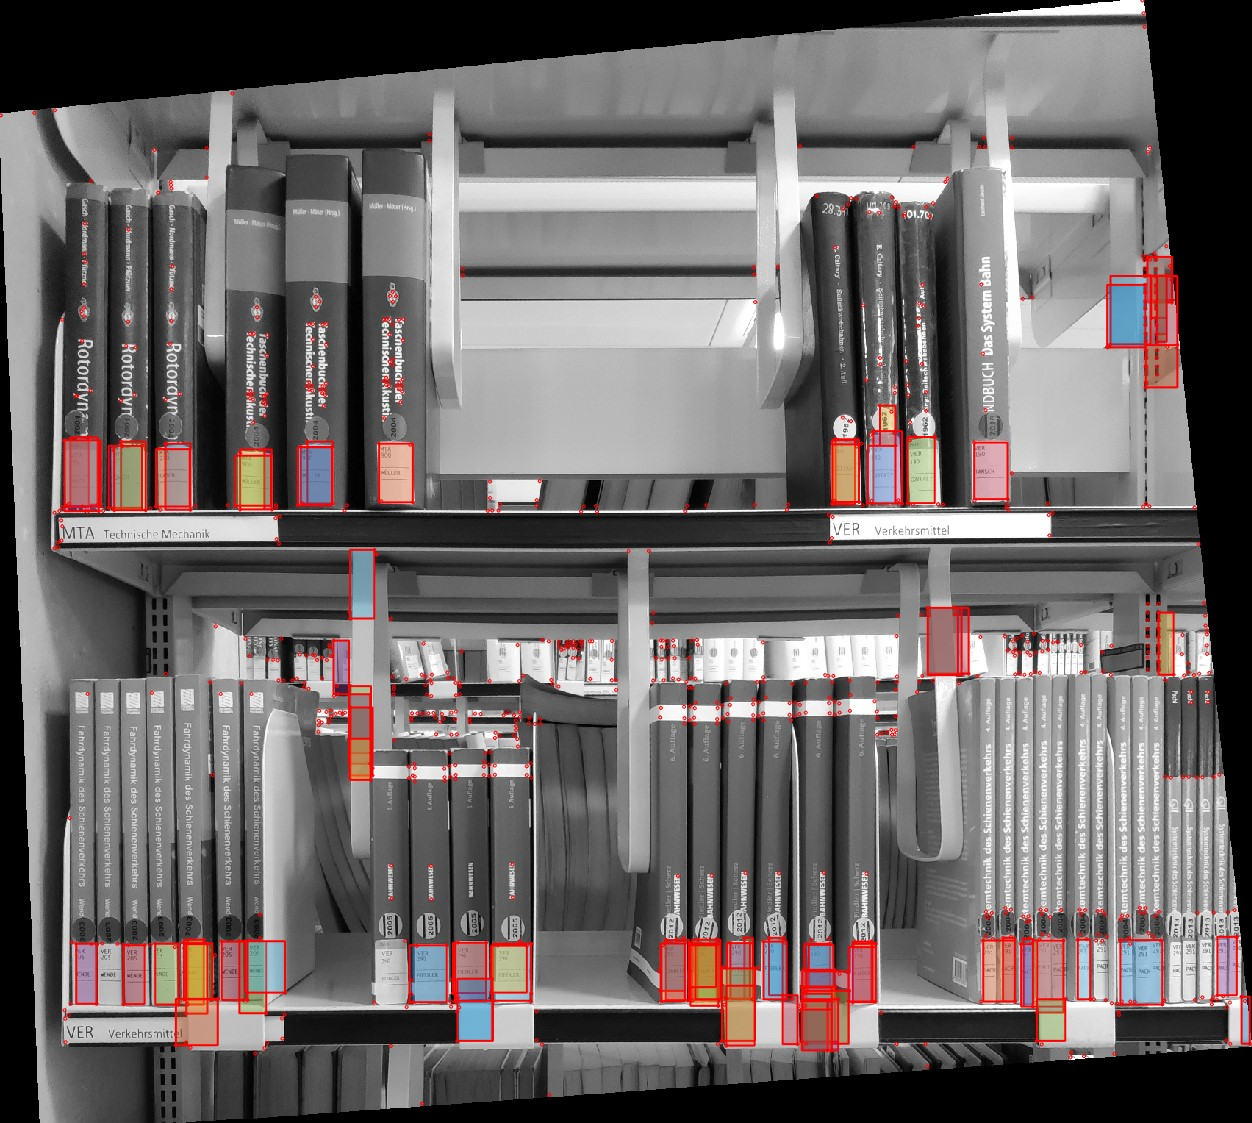
\includegraphics[width=0.4\textwidth]{label_det.jpg}
 \caption{Erkannte Labels}
 \label{fig:img}
\end{figure}
		  
	\item \textit{Werden die Labels korrekt in Bücher-Koordinaten umgewandelt?}\\
		  Bücher werden aufgrund ihrer Labelkoordinaten in Zeilen einsortiert. Im Ergebnisdatensatz wird jedoch nicht mehr zwischen den einzelnen Regalfächern unterschieden, es werde nur die Bounding Boxes der Labels zurückgegeben.
		  
	\item \textit{Werden die Labels der TU-Bibliothek korrekt gelesen und in Text umgewandelt?}\\
		  Aufgrund der vielen False-positives aus dem vorherigen Schritt und der hohen Variabilität der einzelnen Zeichen auf dem Bild, erhalten wir oft zu viele, zu wenige, oder gar die falschen Zeichen.\\(Sehr beliebt sind "Y\dq  und "L" was falsche Zeichen angeht).
		  
	\item \textit{Wird die Wahrscheinlichkeit der Label-Korrektheit angemessen berechnet?}\\
		  Unsere OCR-Implementierung returniert keine zuverlässigen Konfidenzwerte, weshalb es uns nicht möglich war die Korrektheit der Labels bzw. Buchstaben/Zahlen aufgrund dieser Eigenschaft zu messen. Die Konfidenzwerte hatten eine zu niedrige Variabilität und dadurch konnte kein genereller Threshold für das Akzeptieren bzw. Verweigern von Labels gefunden werden. Die Konfidenz war immer im gleichen Bereich, auch bei offensichtlich falschen Resultaten.
		  
\end{itemize}
\subsection{Generelle Evaluierung}
Wir erhalten bei keinem Bild wirklich korrekte Ergebnisse. Je gerader das Bild und je stärker der Kontrast der Etiketten ist desto besser sind die Ergebnisse, jedoch erhalten wir dennoch viele falsche Zeichen vom OCR. Ein großes Upgrade wäre vermutlich noch den deterministischen OCR durch einen Machine-learning Algorithmus zu ersetzen, beziehungsweise die Templates noch etwas anzupassen.\\

\textbf{Die einzelnen Module}\\
Die einzelnen Module sind so aufgebaut, dass sie nicht direkt voneinander abhängen. Jedoch müssen die jeweiligen Vorbedingungen stets erfüllt sein.\\

\textbf{Perpsektivenkorrektur}\\
Die Perspektivenkorrekt funktioniert bei allen Bildern im Datensatz relativ gut. Wichtig ist hier jedoch dass die Bilder in der richtigen Orientierung geladen werden.\\

\textbf{Label Erkennung}\\
Wenn ein Bild mit minimaler perspektivischer Verzerrung eingespeist wird, dann funktioniert die Labelerkennung nominal. Je besser der Kontrast, desto besser die Ergebnisse.\\

\textbf{OCR}\\
Der OCR benötigt ein bild von einem möglichst unverzerrtem Label mit gutem Kontrast und einer guten Auflösung.\\

%%------------------------------------------------------

%%------------------------------------------------------
\section{Schlusswort}
Unser EDBV-Projekt hat uns mit vielen, unterschiedlichen Problemstellungen konfrontiert. Vom korrekten Datensatz bis hin zur Optimierung mussten wir mit originellen und bestehenden Ideen, die auf unser gewähltes Programm zugeschnitten werden mussten, arbeiten. Letztdendlich konnten wir jedoch den Großteil unserer Evaluationsfragen erarbeiten und schließlich beantworten. Die Herausforderungen bestanden hauptsächlich darin, sich eine sinnvolle Struktur - sowohl organisatorisch, als auch implementierungstechnisch - auszudenken und weiters mit Problemen, die spezifisch in unserem Program und mit unseren Datensätzen auftreten zu analysieren und zu beheben. Zum Schluss wollen wir herausheben, dass die Erfahrungen, die wir gemacht haben, sowohl unsere Theorie- und Implementierungskentnisse, als auch Teamarbeit und Kommunikationsskills gestärkt haben.
%%------------------------------------------------------

%%------------------------------------------------------
\bibliographystyle{plain}
\bibliography{edbv_lit}
%%Bei verwendung von Latex schreibt ihr eure Referenzen in ein eigenes bib-File (siehe hier edbv_lit.bib). Jene Referenzen, die ihr im Bericht mittels \cite zitiert, werden automatisch in die Referenzliste übernommen. Weitere Information zum Einbinden von BibTex gibt es hier: http://www.bibtex.org/Using/de/
%%------------------------------------------------------

\end{document}
\grid
\grid
